% This is "sig-alternate.tex" V2.1 April 2013
% This file should be compiled with V2.5 of "sig-alternate.cls" May 2012
%
% This example file demonstrates the use of the 'sig-alternate.cls'
% V2.5 LaTeX2e document class file. It is for those submitting
% articles to ACM Conference Proceedings WHO DO NOT WISH TO
% STRICTLY ADHERE TO THE SIGS (PUBS-BOARD-ENDORSED) STYLE.
% The 'sig-alternate.cls' file will produce a similar-looking,
% albeit, 'tighter' paper resulting in, invariably, fewer pages.
%
% ----------------------------------------------------------------------------------------------------------------
% This .tex file (and associated .cls V2.5) produces:
%       1) The Permission Statement
%       2) The Conference (location) Info information
%       3) The Copyright Line with ACM data
%       4) NO page numbers
%
% as against the acm_proc_article-sp.cls file which
% DOES NOT produce 1) thru' 3) above.
%
% Using 'sig-alternate.cls' you have control, however, from within
% the source .tex file, over both the CopyrightYear
% (defaulted to 200X) and the ACM Copyright Data
% (defaulted to X-XXXXX-XX-X/XX/XX).
% e.g.
% \CopyrightYear{2007} will cause 2007 to appear in the copyright line.
% \crdata{0-12345-67-8/90/12} will cause 0-12345-67-8/90/12 to appear in the copyright line.
%
% ---------------------------------------------------------------------------------------------------------------
% This .tex source is an example which *does* use
% the .bib file (from which the .bbl file % is produced).
% REMEMBER HOWEVER: After having produced the .bbl file,
% and prior to final submission, you *NEED* to 'insert'
% your .bbl file into your source .tex file so as to provide
% ONE 'self-contained' source file.
%
% ================= IF YOU HAVE QUESTIONS =======================
% Questions regarding the SIGS styles, SIGS policies and
% procedures, Conferences etc. should be sent to
% Adrienne Griscti (griscti@acm.org)
%
% Technical questions _only_ to
% Gerald Murray (murray@hq.acm.org)
% ===============================================================
%
% For tracking purposes - this is V2.0 - May 2012

\documentclass{sig-alternate-05-2015}
\usepackage{graphicx}
\usepackage{todonotes}
\usepackage{subcaption}
\usepackage{microtype}
\usepackage{color}
\linespread{0.93}

\begin{document}

% Copyright
\setcopyright{acmcopyright}
%\setcopyright{acmlicensed}
%\setcopyright{rightsretained}
%\setcopyright{usgov}
%\setcopyright{usgovmixed}
%\setcopyright{cagov}
%\setcopyright{cagovmixed}


% DOI
\doi{10.475/123_4}

% ISBN
\isbn{123-4567-24-567/08/06}

%Conference
\conferenceinfo{PLDI '13}{June 16--19, 2013, Seattle, WA, USA}

\acmPrice{\$15.00}

%
% --- Author Metadata here ---
\conferenceinfo{WOODSTOCK}{'97 El Paso, Texas USA}
%\CopyrightYear{2007} % Allows default copyright year (20XX) to be over-ridden - IF NEED BE.
%\crdata{0-12345-67-8/90/01}  % Allows default copyright data (0-89791-88-6/97/05) to be over-ridden - IF NEED BE.
% --- End of Author Metadata ---

\title{Is Readability a Valuable Signal for Hashtag Recommendations?}

%
% You need the command \numberofauthors to handle the 'placement
% and alignment' of the authors beneath the title.
%
% For aesthetic reasons, we recommend 'three authors at a time'
% i.e. three 'name/affiliation blocks' be placed beneath the title.
%
% NOTE: You are NOT restricted in how many 'rows' of
% "name/affiliations" may appear. We just ask that you restrict
% the number of 'columns' to three.
%
% Because of the available 'opening page real-estate'
% we ask you to refrain from putting more than six authors
% (two rows with three columns) beneath the article title.
% More than six makes the first-page appear very cluttered indeed.
%
% Use the \alignauthor commands to handle the names
% and affiliations for an 'aesthetic maximum' of six authors.
% Add names, affiliations, addresses for
% the seventh etc. author(s) as the argument for the
% \additionalauthors command.
% These 'additional authors' will be output/set for you
% without further effort on your part as the last section in
% the body of your article BEFORE References or any Appendices.

\numberofauthors{2} %  in this sample file, there are a *total*
% of EIGHT authors. SIX appear on the 'first-page' (for formatting
% reasons) and the remaining two appear in the \additionalauthors section.
%
\author{
% You can go ahead and credit any number of authors here,
% e.g. one 'row of three' or two rows (consisting of one row of three
% and a second row of one, two or three).
%
% The command \alignauthor (no curly braces needed) should
% precede each author name, affiliation/snail-mail address and
% e-mail address. Additionally, tag each line of
% affiliation/address with \affaddr, and tag the
% e-mail address with \email.
%
% 1st. author
\alignauthor
Ion Madrazo Azpiazu\\
       \affaddr{Computer Science Dept.}\\
       \affaddr{Boise State University}\\
       \affaddr{Boise, Idaho, USA}\\
	   \affaddr{ionmadrazo@boisestate.edu}\\
% 2nd. author
\alignauthor
Maria Soledad Pera\\
       \affaddr{Computer Science Dept.}\\
       \affaddr{Boise State University}\\
       \affaddr{Boise, Idaho, USA}\\
       \affaddr{solepera@boisestate.edu}\\
%
}
% There's nothing stopping you putting the seventh, eighth, etc.
% author on the opening page (as the 'third row') but we ask,
% for aesthetic reasons that you place these 'additional authors'
% in the \additional authors block, viz.
\date{}
% Just remember to make sure that the TOTAL number of authors
% is the number that will appear on the first page PLUS the
% number that will appear in the \additionalauthors section.

\maketitle
\begin{abstract}
%Readability assessment has been successfully applied in many educational-related tasks. However, applications outside this domain are few. 
We present an initial study examining the benefits of incorporating readability indicators in social network-related tasks. 
In order to do so, we introduce TweetRead, a readability assessment tool specifically designed for Twitter and use it to inform the hashtag prediction process, highlighting the importance of a readability signal in recommendation tasks.
\end{abstract}
%
% The code below should be generated by the tool at
% http://dl.acm.org/ccs.cfm
% Please copy and paste the code instead of the example below. 
%
 \begin{CCSXML}
<ccs2012>
<concept>
<concept_id>10003120.10003130.10003131.10003270</concept_id>
<concept_desc>Human-centered computing~Social recommendation</concept_desc>
<concept_significance>500</concept_significance>
</concept>
<concept>
<concept_id>10003120.10003130.10003131.10003292</concept_id>
<concept_desc>Human-centered computing~Social networks</concept_desc>
<concept_significance>500</concept_significance>
</concept>
</ccs2012>
\end{CCSXML}

\ccsdesc[500]{Human-centered computing~Social recommendation}
\ccsdesc[500]{Human-centered computing~Social networks}

%
% End generated code
%

%
%  Use this command to print the description
%
\printccsdesc

% We no longer use \terms command
%\terms{Theory}

\keywords{Hashtag Recommendation; Readability}

\section{Introduction}

Readability is a measure of the ease with which a text can be read. Usually represented by a number, it is an indicator used by teachers to classify and find appropriate resources for students. Several studies have demonstrated the benefits of using readability indicators in educational-related applications, %demonstrating its applicability in tasks 
such as book recommendation, text simplification, or automatic translation. However, applying readability indicators outside this environment remains relatively unexplored. Social networks could benefit from readability assessment. Twitter is a social network where users and texts are the main focus. For this reason, it is natural to think that for Twitter the ease with which a tweet can be understood by a user may affect his interest in it, and therefore influence actions taken, such as re-tweeting, giving a like or replying to the tweet. 

The authors of \cite{age} examined the degree to which the age of a user, a feature strongly correlated with readability, influences who people follow on Twitter, and demonstrated that Twitter users have a higher chance to follow people of similar age.
Using standard readability measures in text from Twitter, which constrains tweets to be of at most 140 characters in length, is not a trivial task. The lack of structure and shortness of those texts make standard natural language analysis techniques inefficient. With that in mind, we developed TweetRead, a novel readability assessment tool specifically designed for tweets. TweetRead takes advantage of social information, such as hashtags or mentions, for predicting the text complexity levels of tweets. Furthermore, in order to highlight the usefulness of such a tool in social networking environments, we developed a simple, yet effective, hashtag recommendation strategy that takes advantage of TweetRead-generated complexity levels of tweets to inform the hashtag recommendation process. 


\section{TweetRead}
TweetRead's goal is to estimate readability of any given tweet $T$. TweetRead is based on a logistic regression technique\footnote{We empirically verified that among numerous supervised techniques, logistic regression was the most promising one.} that fuses simple indicators describing $T$ from different perspectives and determines its text complexity. The indicators considered by TweetRead include: (i) $T$'s readability level, estimated using $Flesch$\footnote{Flesch estimates the readability of a text/tweet $t$, by examining its length and the average length of terms in $t$.} \cite{Fle48}, (ii) $T$'s similarity with respect to word distributions generated from a large Twitter corpora $C$ labeled by age groups, (iii) average readability of each hashtag $h$ in $T$, computed based on the average readability levels estimated using Flesch of tweets in $C$ that include $h$, (iv) average readability level of users mentioned on $T$, estimated using Flesch on tweets written by mentioned users, and (v) frequency of mentions, emoticons, and hashtags in~$T$. 
%\begin{itemize}
%\item Flesch \cite{Fle48} readability score, consisting of a weighted sum of the average length of a terms in the tweet and average length of sentence.
%\item Cosine similarity between tf-idf values of a tweet and the all the tweets for each readability level
%\item Average readability of hashtags in the tweet, considering the readability of a hashtag the average Flesch readability of the tweets it is present on.
%\item Average readability of users mentioned on tweet
%\item Frequency of mentions, emoticons and hash-tags on the tweet
%\end{itemize}

Unlike traditional readability formulas that tend to map readability levels with school grades, to tailor TweetRead to the Twittersphere, we consider six levels of text complexity following Levinston's \cite{develop} adult development stages.

\section{Hashtag Recommendation}
Hashtags are character strings used to represent concepts on Twitter, starting with a \# symbol. They are a core Twitter feature and serve classification and search purposes. Their unrestricted nature, however, creates difficulties, including the fact that the same concept can be represented by different hashtags, hindering the search process of a concept \cite{hashtagRec}. For example, tweets related to the Monaco Formula 1 Grand Prix can be searched using \#monacoGP, \#monacoF1GP or \#monacoF1 retrieving different results. Hashtag recommendation aims at identifying suitable hashtags a user can include in his tweet to reduce the space of tags generated \cite{hashtagRec} and facilitate the ease with which he and other users can locate the corresponding tweet. 

%Hashtag recommendation aims at identifying suitable hasthgs as user can include in his tweet showing the user relevant currently existing hashtags, so that he can re-use them and therefore reduce the space of tags generated \cite{hashtagRec}

Given that (i) the scope of this paper is to validate the importance of considering a text complexity signal to enhance a recommendation task and (ii) multiple and increasingly complex systems have been developed for hashtag recommendation \cite{lda}, we base our study on an existing framework for hashtag recommendation presented in \cite{hashtagRec}. Given a tweet $T$, the proposed framework identifies existing hashtags to recommend by following two major steps: (1) generate candidate hashtags by recommending hashtags present in similar tweets, using tf-idf based cosine similarity and (2) rank hashtags from retrieved candidate tweets using different strategies. The strategies presented in \cite{hashtagRec} include: 
\begin{itemize}
\item \textbf{Similarity}. Prioritizes hashtags included on tweets that have the closes similarity to $T$, as estimated using the well-known tf-idf and cosine similarity measure. 
\item \textbf{Global popularity}. Prioritizes hashtags based on their respective frequency of occurrence on Twitter. 
\item \textbf{Local popularity}. Prioritizes hashtags based on their frequencies of occurrence among the tweets retrieved in response to $T$. 
\end{itemize}

We enhance the proposed strategies by taking advantage of TweetRead, as follows:
\begin{itemize}
\item \textbf{TweetRead}. Prioritizes candidate hashtags that have the same or similar text complexity (estimated using TweetRead) with respect to $T$.
\item \textbf{PopularityTweetRead}. Prioritizes hashtags based on their frequencies of occurrence among Twitter users whose reading abilities are estimated to match $T$'s.
\item \textbf{SimilarityTweetRead}. Prioritizes candidate hashtags based on their respective ranking scores computed using a linear combination of the scores yielded using Similarity and TweetRead. 
\end{itemize}

\section{Initial Assessment}
In this section, we discuss an initial evaluation on TweetRead, as well as its applicability for suggesting hashtags.

\textbf{TweetRead}. Given that readability of social content is an unexplored area, benchmark datasets that can be used for evaluation purposes are unavailable. For this reason, we built our own dataset. We initially gathered 172M tweets over an 8-month period using Twitter streaming API. For the purpose of this experiment we assume that the age of people exactly corresponds to their readability level, and that each tweet written by a user will have the same readability level as its author. With that in mind, we followed the framework presented in \cite{age}, which examines patterns such as ``happy xth birthday", for determining the age of Twitter users. In doing so, we eliminated from our dataset, users (and their corresponding tweets) from whom age  could not be determined. Thereafter, we grouped labeled tweets into 6 age groups, which translates into a uniformly distributed dataset of 22k tweets with their corresponding readability levels. %For evaluating the performance of TweetRead 
We followed a 10-cross-fold validation strategy and measured the accuracy of the predicted readability levels with respect to the ground truth. 
%22k tweets 1609 users
%81 27
As shown in Table \ref{tab:read}, TweetRead significantly outperforms the baselines considered for this assessment: Flesch \cite{Fle48} and Spache \cite{spache1953new}, which are two well-known, traditional readability measures. The reported results demonstrate the need for readability strategies that examine information beyond standard text analysis, if they are meant to be successfully used in the social networking context.

\begin{table}[]
\centering
\begin{tabular}{|c|c|c|}
\hline
Flesch & Spache & TweetRead \\ \hline
27\% & 31\% & 81\% \\ \hline
\end{tabular}
\caption{Performance evaluation of TweetRead vs. baselines.}
\label{tab:read}
\vspace{-0.5cm}
\end{table}

\textbf{Hashtag recommendation}. For evaluating the strategies for hashtag recommendation presented in Section 3, we used the aforementioned dataset. We treated the hashtag of each corresponding tweet as the ground truth. In other words, for each tweet $T$, we generated the corresponding top-N hashtag recommendations and considered relevant the ones matching the hashtags in $T$. As in \cite{hashtagRec}, we used the recall measure to evaluate performance and determine to which  extend the correct hashtags were recommended within the top N generated suggestions.
%For each tweet, containing at least one hashtag, we considered those hashtags as ground truth and top N hashtag recommendations were computed. Same as in \cite{hashtagRec} recall measure was used to evaluate performance, determining with it to what extend where the correct hashtags recommended in the top N.
As shown in Figure \ref{fig:comparison}, even if readability on its own is not a sufficient factor to suggest hashtags, when combined in-tandem with other content-based and/or popularity strategies, it leads to the improvement of the overall hashtag recommendation process. %it is a good complement to other strategies, improving the results when combined with both popularity and similarity metrics.
\begin{figure}[h]

\centering
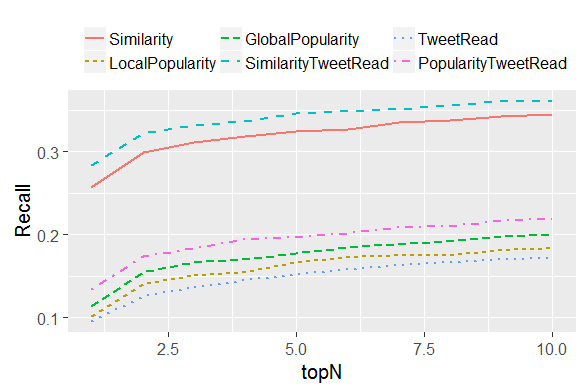
\includegraphics[width=0.48\textwidth]{comparison}
\caption{Hashtag recommendation assessment.}
\label{fig:comparison}
\vspace{-0.5cm}
\end{figure}
% assessment of hashtag recommendation, table comparison each metric\\

\section{Conclusion and Future Work}
In this paper, we presented TweetRead, a novel readability assessment tool specifically designed to predict the readability of tweets. We also discussed the initial study conducted to demonstrate the benefit of using a readability signal in the hashtag recommendation task, which yielded promising results.
In the future, we plan to explore other applications of readability in social networks, such as user recommendation, advertisement targeting or re-tweet prediction. We will also explore techniques to further enhance TweetRead and adapt it to other social networks beyond Twitter.

%
% The following two commands are all you need in the
% initial runs of your .tex file to
% produce the bibliography for the citations in your paper.
\bibliographystyle{abbrv}
\bibliography{sigproc}  % sigproc.bib is the name of the Bibliography in this case
% You must have a proper ".bib" file
%  and remember to run:
% latex bibtex latex latex
% to resolve all references
%
% ACM needs 'a single self-contained file'!
%

\end{document}
